%!TEX root = Journal.tex
% conclusions

\subsection{Transmission System Problem}
The TS has a network of transmission lines and buses. Traditional and renewable generation units, loads and MGs are connected to different buses in the network. The TS solves a day ahead market unit commitment problem, which is a co-optimization of the energy market and ancillary service market. For the energy market optimization, the TS tries to minimize the cost of meeting the system demand with its own generation or energy from MGs. For the ancillary service market optimization, the TS minimizes the cost of providing enough reserve to account for the renewable forecast uncertainty. The reserve service could either come from the TS generator's reserve or the MG's DR. The TS objective function minimizes the energy and ancillary service cost at the same time.  

\subsection{Microgrid Problem}
The microgrid has an aggregated dispatchable load and an aggregated non-dispatchable load, an energy storage unit, and a distributed generation. In the day-ahead market, the MG solves an optimal dispatch problem. The dispatchable load is optimized at some point in between its upper and lower bound. The difference between the upper/lower bound and its set point could be used to provide upward/downward DR. The objective of the MG is to minimize the cost of meeting its demand either by its distributed generation or importing power from the TS and maximize the revenue of providing DR

\subsection{Co-operation Mode}
The TS and MG could work in two modes. The first mode is standalone mode, in which the two systems are totally separated from each other. In this mode, the two systems could not exchange energy and the MG could not provide DR to the TS. The second mode in co-optimization mode. Under our bilevel optimization framework, the TS decides the price of MG energy import and export as well as the price for purchasing MG DR, the MG responds to those prices by exchanging a certain amount of energy with the TS and selling a certain amount of DR to the TS.

The co-optimization between the TS and MG is illustrated in Fig.~\ref{wees}
\begin{figure}[H]
\centering
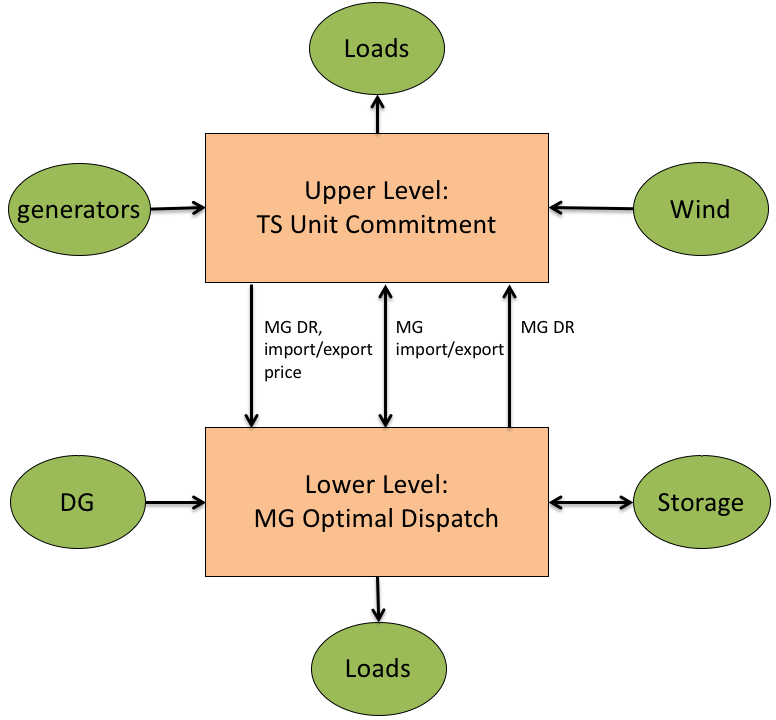
\includegraphics[scale=0.35]{flowc.png}
\caption{Co-optimization between the TS and MG}
\label{wees}
\end{figure}

\subsection{Renewable Forecast Uncertainty Management}
In this work, we use a robust approach to manage the uncertainty in renewable forecast. Specifically, for a renewable generation forecast and a set of possible generation scenarios, we calculate the upward/downward forecast deviation by taking the difference of the hourly maximum/minimum generation scenario and the hourly forecast. The downward/upward TS generation reserve and upward/downward MG DR are used to account for the upward/downward renewable forecast deviation.

